%!TEX root = ../tesis.tex
\subsection{Identificación de focos de infestación del dengue}
\label{sec:cap4-identificacion-focos}
Las metodologías de vigilancia entomológica basadas en la distribución geográfica de larvitrampas
u ovitrampas, como las presentadas en
\cite{NINO2011,petric2012surveillance, journal.pone.0054167,nino2008uso}, permiten generar
información regionalizada sobre la abundancia poblacional del vector. Los datos
sobre los mosquitos recolectados deben mantenerse para crear un registro histórico de las
especies de mosquitos que se encuentran en asociación con diferentes hábitats y patógenos para
permitir la detección temprana de las adaptaciones \cite{petric2012surveillance}.

En \cite{NINO2011} se propone una metodología de vigilancia entomológica basada en la utilización
de larvitrampas para la identificación de focos de infestación del dengue, donde las larvitrampas
deben ser distribuidas geográficamente (\figref{fig:sig-distribucion-puntos-control}) para generar
información regionalizada correspondiente al área de estudio. Las técnicas de
interpolación espacial permiten transformar la información regionalizada en mapas de
interpolación (\figref{fig:sig-puntos-control-interpolacion}), donde se puede apreciar los niveles
de infestación del vector del dengue, y el riesgo correspondiente a la abundancia de mosquitos
observada en el área de estudio \cite{NINO2011}. El hecho de contar con esta información
regionalizada permitirá a las autoridades pertinentes definir y planificar mejor las medidas de
prevención y control a realizarse para reducir los niveles de infestación en las zonas criticas
\cite{NINO2011, nino2008uso, petric2012surveillance}.


\begin{figure}[!htbp]
    \centering
    \begin{subfigure}[b]{0.45\textwidth}
        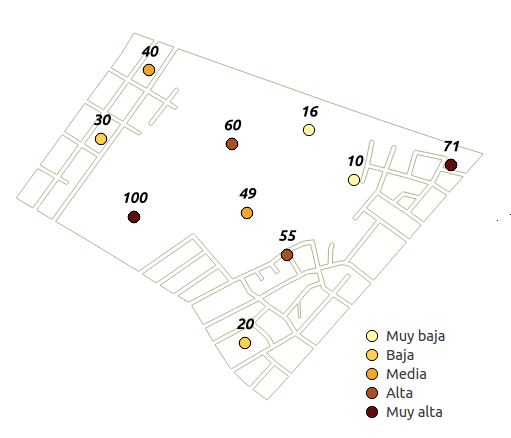
\includegraphics[width=1\textwidth]{capitulo-2/graphics/distribucion-puntos-control.png}
        \caption{\label{fig:sig-distribucion-puntos-control}Ejemplo de disposición de larvitrampas y abundancia de larvas.}
    \end{subfigure}
    ~~~~
    \begin{subfigure}[b]{0.45\textwidth}
        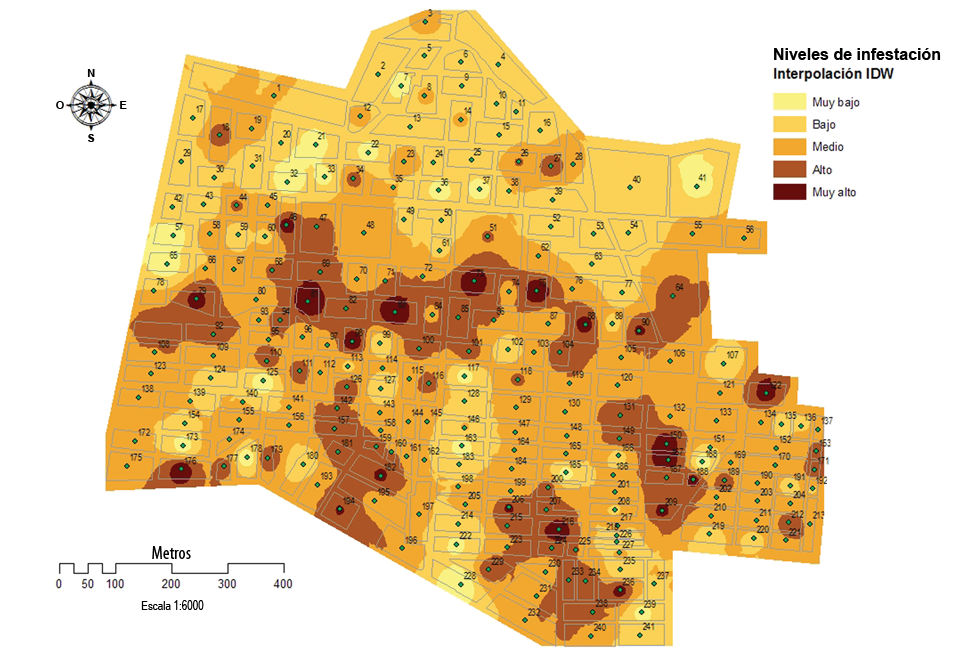
\includegraphics[width=1\textwidth]{capitulo-2/graphics/puntos-control-interpolacion.png}
        \caption{\label{fig:sig-puntos-control-interpolacion} Ejemplo de mapa de interpolación resultante.}
    \end{subfigure}
\end{figure}

Los mapas de interpolación resultantes, indican, con mayor detalle que los índices aédicos
tradicionales, los lugares específicos donde sería necesario tomar medidas de prevención y
control de acuerdo al grado de infestación, permitiendo así una mayor racionalización de tiempo y
recursos \cite{NINO2011}.
